\documentclass[12pt,oneside]{book}
\usepackage{times,mathptmx}
\usepackage[pdftex]{graphicx}
\usepackage{calc}
\usepackage{tabularx,ragged2e,booktabs,caption,subcaption}
\usepackage{array}
\newcolumntype{L}[1]{>{\raggedright\let\newline\\\arraybackslash\hspace{0pt}}m{#1}}
\newcolumntype{C}[1]{>{\centering\let\newline\\\arraybackslash\hspace{0pt}}m{#1}}
\newcolumntype{R}[1]{>{\raggedleft\let\newline\\\arraybackslash\hspace{0pt}}m{#1}}
\usepackage{multirow}
\usepackage{tocloft}
\usepackage{xcolor}
\usepackage{color,soul}
\usepackage{amsmath}
\definecolor{linknavy}{rgb}{0,0,0.50196}
\definecolor{linkred}{rgb}{1,0,0}
\definecolor{linkblue}{rgb}{0,0,1}
\usepackage{float}
\usepackage{graphpap}
\usepackage{rotating}
\usepackage{graphicx}
\usepackage{geometry}
\usepackage{relsize}
\usepackage{ltablex}
\usepackage{longtable}
\usepackage{lscape}
\usepackage{amssymb}
\usepackage{makeidx} % Create index at end of document
\usepackage[nottoc,notlof,notlot]{tocbibind} % Put the bibliography and index in the ToC
\usepackage{lastpage} % Automatic last page number reference.
\usepackage[T1]{fontenc}
\usepackage{enumerate}
\usepackage{upquote}
\usepackage{moreverb}
\usepackage{xfrac}
\usepackage{cite}
\usepackage{tikz}
% \usepackage{subfig}
% \usepackage{caption}
\usepackage[toc,page]{appendix}
\usepackage{notoccite}
\usepackage{colortbl}
\usepackage{titlesec}
\titleformat{\chapter}[hang] 
{\normalfont\huge\bfseries}{\chaptertitlename\ \thechapter}{1em}{} 
\titlespacing*{\chapter}{0pt}{-30pt}{20pt}

\newcommand{\nopart}{\expandafter\def\csname Parent-1\endcsname{}} % To fix table of contents in pdf.

\usepackage{siunitx}
\sisetup{
    detect-all = true,
    input-decimal-markers = {.},
    input-ignore = {,},
    inter-unit-product = \ensuremath{{}\cdot{}},
    multi-part-units = repeat,
    number-unit-product = \text{~},
    per-mode = fraction,
    separate-uncertainty = true,
}

\usepackage{listings}
\usepackage{textcomp}
\definecolor{lbcolor}{rgb}{0.96,0.96,0.96}

\usepackage[pdftex,
        colorlinks=true,
        urlcolor=linkblue,     % \href{...}{...} external (URL)
        citecolor=linkred,     % citation number colors
        linkcolor=linknavy,    % \ref{...} and \pageref{...}
        pdfproducer={pdflatex},
        pdfpagemode=UseNone,
        bookmarksopen=true,
        plainpages=false,
        verbose]{hyperref}

\setlength{\textwidth}{6.5in}
\setlength{\textheight}{9.0in}
\setlength{\topmargin}{0.in}
\setlength{\headheight}{0.pt}
\setlength{\headsep}{0.in}
\setlength{\parindent}{0.0in}
\setlength{\itemindent}{0.25in}
\setlength{\oddsidemargin}{0.0in}
\setlength{\evensidemargin}{0.0in}
% \setlength{\leftmargini}{\parindent} % Controls the indenting of the "bullets" in a list
\setlength{\cftsecnumwidth}{0.45in}
\setlength{\cftsubsecnumwidth}{0.5in}
\setlength{\cftfignumwidth}{0.45in}
\setlength{\cfttabnumwidth}{0.45in}
\setlength{\parskip}{1em}

\newcommand{\titlesigs}
{
\large
\flushright{UL Firefighter Safety Research Institute\\
{\em Stephen Kerber, Director} \\
\hspace{1in} \\
}
}

\newcommand{\headerB}[1]{
\flushleft{
\fontsize{28}{33.6}\selectfont
\bf{#1}
}
}

\newcommand{\headerC}[1]{
\vspace{.5in}
\flushright{\fontsize{14}{16.8}\selectfont
#1}
}

% \newcolumntype{L}{>{\centering\arraybackslash}m{4cm}}

\floatstyle{boxed}
\newfloat{notebox}{H}{lon}
\newfloat{warning}{H}{low}

\newenvironment{conditions}
  {\par\vspace{\abovedisplayskip}\noindent\begin{tabular}{>{$}l<{$} @{${}={}$} l}}
  {\end{tabular}\par\vspace{\belowdisplayskip}}


\usepackage{longtable}

\usepackage{fancyhdr}
\pagestyle{fancy}
\lhead{}
\rhead{}
\chead{}
\renewcommand{\headrulewidth}{0pt}

\setcounter{secnumdepth}{0}

\begin{document}
\pagenumbering{gobble}

\frontmatter

\begin{minipage}[t][9in][s]{6.25in}

\headerB{\ul{
Tech Panel Comments \& Responses
}}

\vspace{0.5in}

\headerB{
Impact of Fire Attack Utilizing \\
Interior and Exterior Streams on\\ 
Firefighter Safety and Occupant \\
Survival: Water Mapping\\
}

\vspace{1.5in}

\today

\normalsize

\headerC{
{
\flushleft{
\vspace{0.2in}
Craig Weinschenk \\
Keith Stakes \\
Robin Zevotek \\
UL Firefighter Safety Research Institute \\
Columbia, MD 21045 \\
\vspace*{2\baselineskip}

}

\vfill

\flushright{


\includegraphics[width=2.in]{Figures/General/FSRI_GraphicShield} \\[.3in]
}
}
}
\end{minipage}

\newpage

\tableofcontents

\newpage

\mainmatter

\chapter*{Background}
\label{background}
\addcontentsline{toc}{chapter}{\nameref{background}}

This document has been created to track and respond to the comments made by the technical panel as part of the UL FSRI DHS 2013 project "Impact of Fire Attack Utilizing Interior and Exterior Streams on Firefighter Safety and Occupant Survival: Water Mapping". 

A special thanks to the individuals listed below who provided feedback to the project team at FSRI. 

\begin{table}[!ht]
	\centering
	\caption*{Fire Service Technical Panel}
	\begin{tabular}{llc}
		\toprule[1.5pt]
		& Name & Fire Department \\ 
		\midrule
		& Steve Brisebois  & Montreal Fire Department \\ 
		& Matt Carrigan    & Montgomery County Fire and Rescue Service \\ 
		& Tony Carroll     & Washington DC Fire Department \\ 
		& Albert Castillo  & Houston Fire Department \\ 
		\checkmark & Chad Christensen & Los Angeles County Fire Department \\ 
		& John Chubb       & Dublin Fire Brigade \\ 		 		  
		& Danny Doyle      & Pittsburgh Fire Department \\ 
		& Aaron Fields     & Seattle Fire Department \\ 
		\checkmark & Jason Floyd      & Las Cruces Fire Department \\ 
		& John Gallagher   & Boston Fire Department \\ 
		& Chad Green       & Anchorage Fire Department \\ 
		\checkmark & Kelly Hanink     & Eden Prairie Fire Department \\ 
		& Samuel Hittle    & Wichita Fire Department \\ 
		& Jacob Hoffman    & Toledo Fire/Rescue Department \\ 
		\checkmark & Josh Hummel      & Howard County Department of Fire and Rescue Services \\ 
		\checkmark & Jerry Knapp      & West Haverstraw (NY) Fire Department \\ 
		\checkmark & Dennis Legear    & Oakland Fire Department \\ 
		\checkmark & Hans Neiling     & Zuid Limburg Fire \\ 
		& Nick Martin      & Columbia Fire Department \\ 
		& Ray McCormack    & Fire Department of New York \\ 
		& John McDonough   & New South Wales Fire Department \\ 
		\checkmark & Jordan Mohr      & Sedgwick County Fire District 1 \\ 
		& Steve Pegram     & Goshen Township Fire and EMS \\ 
		\bottomrule[1.25pt]
	\end{tabular}
	\\ \checkmark~~indicates panel member provided feedback on the water mapping report.
\end{table}

\newpage

\chapter*{Comments and Responses}
\label{comments}
\addcontentsline{toc}{chapter}{\nameref{comments}}

\begin{longtable}{|L{2.6in}|L{2.6in}|c|}

		\toprule[1.5pt]
		Comment/Question & Response & Report Updated \\ 
		\toprule[1.5pt] \endfirsthead
		\toprule[1.5pt]
		Comment/Question & Response & Report Updated \\ 
		\toprule[1.5pt] \endhead
		\midrule
		Is their any CO data for test 3? It says the sensors were not used? Is the data just not loaded yet or was that the burn they were having sensor issues. Sorry can't remember! &
		Comment pertains to Fire Attack report. Added to fire attack report comments list. & \\
		
		\hline
		If I am reviewing things with an open mind and trying to be objective am I correct in that the temps with door control incorporated drop at a quicker rate than without? Between test 2 and 3? & 
		Comment pertains to Fire Attack report. Added to fire attack report comments list. & \\

		\hline
		Overall it also appears that water on the fire regardless of how it was applied improved conditions in the fire room and surrounding areas. Yet the straight stream seems to be most effective. Early water on the fire appears to be best for the victims inside. &
		Comment pertains to Fire Attack report. Added to fire attack report comments list. & \\

		\hline
		CO levels have been a big concern with guys when it comes to door control. Unless I am missing something it seems at least in my first glance, that CO levels in the survivable space are not raising until suppression? Are we making things worse by putting out the fire? It also seems that with door control CO levels didn't rise any more than without? & 
		Comment pertains to Fire Attack report. Added to fire attack report comments list. & \\

		\hline
		To determine the best flow type is the velocity what we should be looking at? & 
		Comment pertains to Fire Attack report. Added to fire attack report comments list. & \\

		\hline
		Figure 5.1 (pg 48) and its associated write-up don't seem to connect exactly. I had to re-read that piece and look at the picture again to understand it. The text states that the dispersion was fairly equally radially to 360 deg with some impact by gravity. But the horizontal arrows (at 90 and 270 deg) are nearly the same as the downward one (280 deg). I just think the arrows need to be depicted a little more accurately to match the words. & 
		Adjusted arrows to ensure the effect of gravity is better depected. & \checkmark \\  

		\hline
		When I read the write-up about Figure 5.2 (pg 49) I thought it was lacking info, which it turns out I found in the section on water distribution in the next section. I don't know if it would be helpful to add text to the water dispersion paragraph to tell the reader about the additional effects of the high angle attack that are described further in the water distribution section or not. That might not be a thing needed in a research report. & 
		Section 5.2 is intended to discuss the dispersion (how the stream breaks up) and section 5.3 discusses how dispersion effects distribution. The idea is to provide building blocks for the reader to put together the pieces. \textbf{Any suggestions on how to clarify this further?} & \\

		\hline
		I feel like the last two rows Table 5.1 (Tactical Choices Summary) present issues. The Nozzle Movement tactical choice states a positive impact for Interior attack from an `O' pattern at the ceiling. But the prior discussion about nozzle movement says "When compared to each other, nozzle movement had little effect on the distribution in the compartment... While the distribution for the fixed pattern was more uniform (flatter)..." Those statements don't appear to match. Further, in the nozzle movement discussion section, there doesn't seem to be any mention of nozzle movement and fog nozzles or any graphs that support the statement in the summary table that an `O' pattern provides good distribution. Or if there is, I didn't make the connection very well so you might want to look to see where things might be restated or tied together better. &
		Changed Nozzle movement to the following "Nozzle movment had little effect on distribution." & \checkmark \\

		\hline 
		Table 5.1 In the Bale Position section, I don't think it's stated that the testing was only tested in the exterior case. Maybe that should be added to help with clarity and completeness and to support the last row of the summary table? &
		Added verbage to Seciton 5.5.2 under bale position to indicate the expeted interior results and adjusted table to match. & \checkmark \\  

		\hline
		I think it's important to include that these findings are purely distribution and not considering air entrainment so conclusions are drawn prematurely by those reading the study. (This could include the 1/2 bale smoothbore technique discussed at the end or even changing the angle of the stream in the window as it relates to air entrainment. I'm not sure if these were all tested in the entrainment piece or not) I can say that I wouldn't have drawn those conclusions as I'm reading the report for what it is, but could see it being a potential issue. & 
		Agreed, added a paragraph to the endo of the discussion section to address this `This section discusses the tactical choices as they relate to water distribition. It is important to understand that water distribution is not the only concern when discussing fire suppression tactical choices. Other considerations, for example air entrainment, may play a role in the nozzle firefighters choice of hose stream. Fire suppression opertaions involve a significant number of varriables, making the system extermely complex. Understanding how the varriables interact is out of the scope of this particular analysis and discussion.' & \checkmark \\

		\hline
		`bale' of a nozzle instead of `bail' & 
		IFSTA references `bale', changed all instances to match. & \checkmark \\

		\hline
		`Freeman' has typo as `Freedman' & 
		corrected typo & \checkmark \\


\end{longtable}
\checkmark~~indicates change made to report to address comment.

% \chapter*{Figures}
% \label{figs}
% \addcontentsline{toc}{chapter}{\nameref{figs}}

% \begin{figure}[H]
% \centering
% 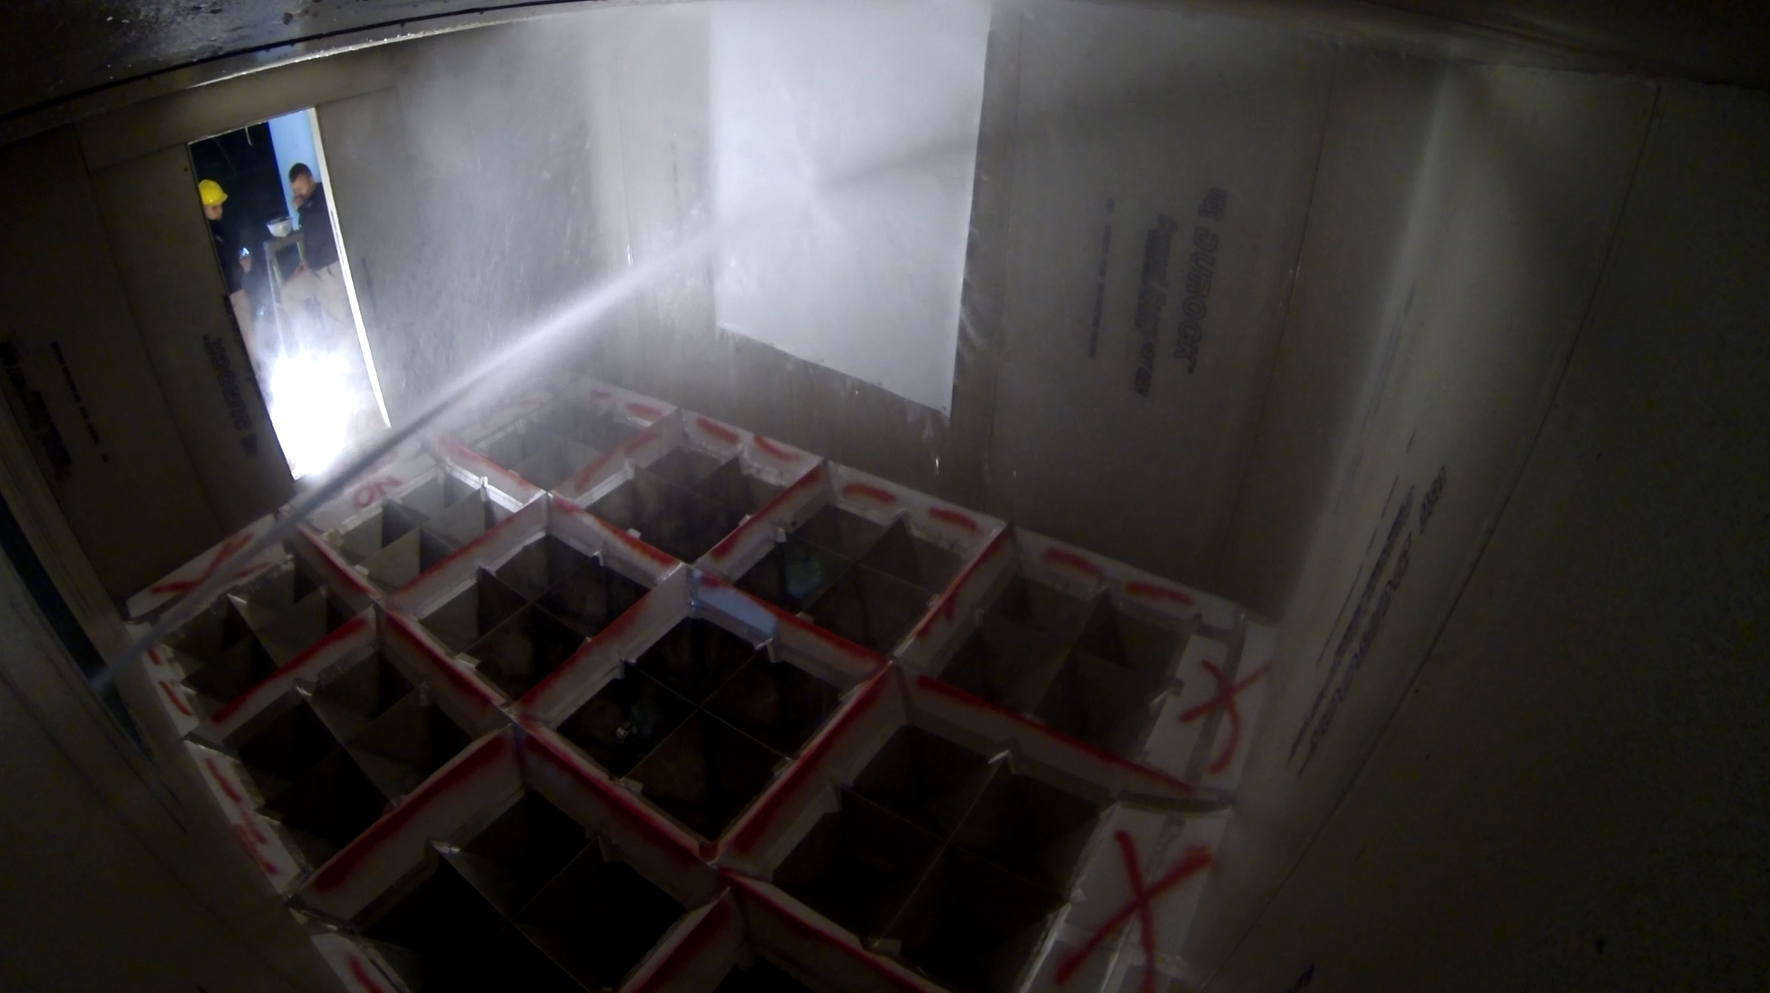
\includegraphics[width=\textwidth]{Figures/Water_Distribution/Nozzle_Directions/Exterior_AtWall_SB.png}
% \caption{Water dispersion of straight stream impacting a wall at an approximate 90$^\circ$ angle}
% \label{fig:at_wall}
% \end{figure}

\newpage

\begin{appendix}

\chapter*{Technical Panel Responses}
\label{panel_responses}
\addcontentsline{toc}{chapter}{\nameref{panel_responses}}

\section{Chad Christensen}

Steve,
 
I hope all is well.  I have been swamped with recruit training and trying to finalize our turnout spec. I know I am preaching to the choir when it comes to being busy.  
 
As we continue in in this process for the Fire Attack study one thing have have not gone on record about is the acquired structure burns.  As is everyone else I am very disappointed to know that we will not be conducting those experiments. I think we may be missing an opportunity to gain further buy in from those around the country that see the tests even though just contents fires being tested in actual structures.  We all know the lab houses are real structures too.  Yet with the opportunity to burn in the concrete buildings we can easily recreate the same environment over and over without worrying about it extending on us or getting away from us.  One of the most effective videos for training transitional attack  has been the video NIST not UL (Robyn corrected me on that at FDIC last year...ooops) with the side by side room showing how air can push products of combustion not fire. My understanding is that was a contents fire too not a structure fire.  We have not been testing structure fires for the first 24 experiments.  Why don't we continue to test contents fires and do the burns?  I know scheduling is crazy and everyone is busy. Just my thoughts and open for discussion between us.  It would allow an opportunity to test different transitional attack methods(flow pause flow pause/ or flow for 10 sec, 20 sec and so on.)  Again just my thoughts and I don't have all the info I am sure with what is needed for you guys to pull of an acquired structure burn in Columbia.   
 
As for the water mapping portion of the study.  Very interesting results.  So I am curious as to what kind of input you are looking for from us.  As I go through the data the biggest things that stick out to me are: 
1 the smooth bore and straight stream are close in effectiveness and that is great because it can be at the choice of the user as to which nozzle they choose. 
2. the steeper the angle you take the more coverage of surfaces you get which will then give you better cooling when applying water from an exterior position.  Along with a better distribution of water if from a fixed position if from the exterior.  
 
These are all things I feel we have been able to see prior to the study from use on the fire ground or training fires. Now we have the data to support or explain what we see.  This will be excellent for reinforcing particulars in the tactical considerations down the road.  To me and I know you know this. It is that this piece by itself is helpful for the fire-ground but it needs the air entertainment to truly go with it side by side.  Air can so negatively effect the fire ground that if it isn't side by side we could make a bad decision and use a fog stream because it effectively covers surfaces. 
 
Below are some questions I put up on the board last year.  Not sure if you guys have the answers to them yet.  I would like to hear your thoughts to them.  I have a few more points that I am digging into a little more and will email you shortly on those items. If you need more input on water mapping please let me know.  
 
 
\begin{enumerate}
\item Is their any CO data for test 3? It says the sensors were not used? Is the data just not loaded yet or was that the burn they were having sensor issues. Sorry can't remember!

\item If I am reviewing things with an open mind and trying to be objective am I correct in that the temps with door control incorporated drop at a quicker rate than without? Between test 2 and 3?

\item Overall it also appears that water on the fire regardless of how it was applied improved conditions in the fire room and surrounding areas. Yet the straight stream seems to be most effective. Early water on the fire appears to be best for the victims inside.

\item CO levels have been a big concern with guys when it comes to door control. Unless I am missing something it seems at least in my first glance, that CO levels in the survivable space are not raising until suppression? Are we making things worse by putting out the fire? It also seems that with door control CO levels didn't rise any more than without?

\item To determine the best flow type is the velocity what we should be looking at?

\end{enumerate}
 
Thanks
 
Chad
 
Chad Christensen \\
Fire Captain \\
Los Angeles County Fire Department \\
Fire Station 18-C \\
310-671-5368 work \\
951-285-3001 cell \\

\section{Kelly Hanink}

Steve,
 
I have reviewed the report.  One general comment is that I found typos, grammatical mistakes, and awkwardly worded statements that need some general editing.  I would be happy to make those markups and provide if that would be helpful.  But I didn't spend the time doing that up front in case that's something that someone is still set to do at the end.  I believed my objective for you was to read for content and ignore those issues.  I'm one of an odd sort in engineering who actually learned something in English class too. So if you need that basic editing, let me know.
 
As far as content goes, I think the report turned out well.  The description of what happens seems clear to me, and the conclusions follow from that.  I think I can see where people's arguments are going to stem with this information, but then once I think I have that figured out someone comes up with something new.  
 
Anyway, I do have a few items that struck me in terms of content presentation:
 
Figure 5.1 (pg 48) and its associated write-up don't seem to connect exactly.  I had to re-read that piece and look at the picture again to understand it.  The text states that the dispersion was fairly equally radially to 360 deg with some impact by gravity.  But the horizontal arrows (at 90 and 270 deg) are nearly the same as the downward one (280 deg).  I just think the arrows need to be depicted a little more accurately to match the words.
 
When I read the write-up about Figure 5.2 (pg 49) I thought it was lacking info, which it turns out I found in the section on water distribution in the next section.  I don't know if it would be helpful to add text to the water dispersion paragraph to tell the reader about the additional effects of the high angle attack that are described further in the water distribution section or not.  That might not be a thing needed in a research report.
 
I feel like the last two rows Table 5.1 (Tactical Choices Summary) present issues.  The Nozzle Movement tactical choice states a positive impact for Interior attack from an 'O' pattern at the ceiling.  But the prior discussion about nozzle movement says "When compared to each other, nozzle movement had little effect on the distribution in the compartment....While the distribution for the fixed pattern was more uniform (flatter)..."  Those statements don't appear to match.  Further, in the nozzle movement discussion section, there doesn't seem to be any mention of nozzle movement and fog nozzles or any graphs that support the statement in the summary table that an O pattern provides good distribution.  Or if there is, I didn't make the connection very well so you might want to look to see where things might be restated or tied together better.  In the Bale Position section, I don't think it's stated that the testing was only tested in the exterior case.  Maybe that should be added to help with clarity and completeness and to support the last row of the summary table?  
 
I think that's it.  I feel like I haven't been nearly as helpful or as engaged as I wanted to be.  I hope that I can do better at least with the phases that remain and beyond.
 
Let me know if you have any questions about any of my comments.
 
Thanks,
Kelly
 
 
Kelly Hanink \\
Assistant Chief of Health \& Safety \\
Eden Prairie Fire Department \\

Cell: 952.946.9951 \\
Office: 952.949.8356 \\

\section{Josh Hummel}

Report looks good to me.  The larger considerations and pulling all of the concepts together will be on the training end of things.  It obviously all gets weighed against the air entrainment results.  Hope I'm not missing major stuff that others may have seen but it all looked appropriate to me. 
 
I think it's important to include that these findings are purely distribution and not considering air entrainment so conclusions are drawn prematurely by those reading the study.  (This could include the 1/2 bale smoothbore technique discussed at the end or even changing the angle of the stream in the window as it relates to air entrainment.  I'm not sure if these were all tested in the entrainment piece or not)  I can say that I wouldn't have drawn those conclusions as I'm reading the report for what it is, but could see it being a potential issue as you guys know all too well from the spin that gets put on every word coming out of your mouths.
 
Only things I saw were a few spelling things that you all may have noted already but I'm anal retentive soooo... 
`bale' of a nozzle instead of `bail' (changed back and forth throughout)
Freeman is referenced as Freedman occasionally
 
Looking forward to seeing the air entrainment results.  Robin said they'd probably be coming shortly after comments on this report.

\makebox[\linewidth]{\rule{\textwidth}{0.4pt}}

I don't know what the conversations have been to the point with you and Dennis, but obviously I received his email.  I agree with many of the elements he thought were interesting as noted in the PDF he supplied.  Not sure if we were supposed to include those things if you wanted them emphasized in the report at all.
 
I understand the necessity of data on water on the fire from inside the compartment.  It's been a point of discussion from the very first meeting and rightfully so as the past study information has been wildly misinterpreted.  However, to me the water mapping and even the air entrainment to a large extent is about the approach to the fire room.  
 
John Chubb broke down the fire attack in three portions:  deploying the line, approach to the fire room, and extinguishment at/in the room. The second segment is where most of us differ and is where this portion of the project falls.  Once we're in the room the water disperses largely where we focus the nozzle, thus the focus on appropriate nozzle techniques by many of the instructors on the panel.  Water movement in angles not tested in the study have to be extrapolated from the findings as every single angle/pressure/flow/movement can't be tested, however it seems the only truly non-tested element in the water mapping seems like it would be water perpendicular to the ceiling in an effort to disperse in multiple directions.  It's already been acknowledged that a future project is expanding on these projects to determine flow of water across the ceiling in larger spaces which would be the other large difference once inside a large room.
 
I'm assuming you guys know this already or feel something similar.  The assertion that we've missed the mark on the testing, especially in this portion, ironically misses the mark itself.  The work done on this project is quality and certainly gives us a more complete picture of what's happening during the interior attack process.  You, Robin, and the whole group seem to not be impact by the critics too much but I wanted to provide a counter argument saying that I believe the tests were not lacking as otherwise argued.  

\section{Dennis Legear}

Steve and Robin:

Below via the drop box link is a scanned copy of the Water Mapping PDF with my hand written notes on it. Steve you know I wanted to go to the water mapping experiments as I have spent a lot of time over my career messing with this concept.

\hyperlink{https://www.dropbox.com/sh/1wmpqxr2a5fow0c/AAB1bfG-yKjGBKFCOlRtaYDya?dl=0}{Dropbox Link}

Please take the time to review my notes on the scanned copy I took the time to read the entire document.  First the positive, I found the no difference between nozzle pressure and distribution a nice confirmation of a sticking point I have with some.  Also that in a residential compartment probably nothing is gained by an exterior 2.5-inch handline 265gpm+ when it is flown from exterior to interior more water into the room sure, but in the exact same place. (less than 400 sq feet compartment)

\textbf{\ul{Now as for the interior attack part, what was done at the water mapping was not an interior attack.}}  It was a interior approach with water flow from before the threshold of the fire compartment.  I find it valuable, however a interior attack is finished with the nozzle in the fire compartment.  This at best is 1/2 a \ul{interior attack}. 

\textbf{\ul{I have a video attached pieces of what I sent to the ULFRSI to define interior attack.}}  Note the flowing approach (which is what the water mapping interior experiment operations is replicating, remote water to cool) and then the nozzles' entry into the "fire compartment".  At the 40sec mark in the attached video see nozzle past the door threshold at the 1:30 mark hear me yelling \textbf{\ul{through the door!}}  I was reinforcing to the students, one must get up and past through the door to properly wet the entire space of the fire compartment.   This was the student's second try at the flowing push.  Only after the nozzle has passed into the fire compartment do you really own the space as far as application of water to the dry side and directly over head (door header block this on approach), a nozzle in the fire compartment (at critical flow) is sole requirement of a successful interior attack.  These full room wetting actions are impossible from the exterior/interior hallway position or outside the door, remote application.  \textbf{\ul{That exterior flow from the hallway is to permit taking the door way, that is all.}} 

I suggest strongly to re-title the document to \textbf{\ul{Exterior Remote Application and Interior Remote Application Water Mapping}} as that is what it is.  Anyone that reads this with fire duty under their belts will come to the same conclusion, in my opinion.  I have never since 1993 every receive instruction to stop short of the fire room, this experiment in my mind shows what happens when you stretch short by a few feet before the fire compartment.  A failure to be able to gain full access to apply water to the entire fire compartment.    

Now I will be gone from 2/19 till 3/23 out of the country.  I discussed all this with the CC'd members of the panel.  Which are the ones I interacted with the most  (I want this shared with all panel members though).  They to my understanding have the same/similar concerns.  

We all also feel that we would like to have you send out a sample of your analysis of two experiments.  \textbf{\ul{To be frank I was overwhelmed could you please send your thoughts on Experiment \#8 Interior vs  Experiment \#20 exterior.}}  

I picked those two as they are the two bedroom fire examples.  Because again as these members are aware it was decided to stick the nozzle through the window without consulting the panel on many of the exterior fire attack tests.  \textbf{\ul{I/We gave up the second story to gain more experiments, but it was stated no nozzle through the window, stick with Governor Island Approaches.}}  

In fact I have no problem with this (nozzle through the window) and instruct that if you apply water through a first story window for what ever reason required it.  After application if possible reach in and coat the room with water hence gaining the sill and getting a interior attack water application.  I am curious what the other CC'd members think?  But in many ways the nozzle at the UL burns through the window had better ability to coat the fire room because of the probes at the end of the hallway, another point that I took issue with.  The hallway door probes were preventing the nozzle team's direct advancement into the fire compartment hence it was not a good interior gold standard attack.   

\textbf{\ul{The issues above I thought would clearly be resolved at the acquired structure burns.}}  Finally note the One Size Does Not fit All transitional attack doc and the Peach Fire video in the drop box link please review .  This "Peach Street" engine company in the video stretched the 1st handline past the closer stairway that leads to the interior 2nd floor apartment door.  They went to the C side to Governor Island style exterior attack.  They picked exterior water over rapid interior water.  I believe the video speaks for itself.  \textbf{\ul{Why did the exterior water fail to change conditions and the fire continue to grow?  Can you provide your thoughts on this video Steve and Robin?}}  

I did wrote this because I have a feeling I will miss the last meeting based on my request for firm dates over the last few months.  Loss of the acquired structure burns where void space spread, and regrowth could have been better quantified was a big impact to this projects ability to succeed.  I suggest applying for another grant and moving forward in the future.  \textbf{\ul{As of now I feel we have missed the mark for whatever reason maybe we did not properly define Interior attack to UL staff,}} because a nozzle through a window is now interior attack for example.  The very reason I was adamant not to allow it, was not because I would not do it or have not done it, but because it is not an exterior attack.  An interior attack is one were the nozzle is in the fire compartment at the end and can coat the entire room with water.  These are my thoughts I still hope to make the final panel meeting.  
Thanks in advance,

Dennis 925-787-6875

\section{Jordan Mohr}

Steve,
 
Everything that I can see from my point of view for the water mapping looks good. The explanation for how the results were recorded, the visual charts and the brief history of how we got to this point really helps the reader understand why these tests were done. I think it was well put together and knowing that this is just a small piece will be beneficial. Personally I feel like newer members to the fire service like myself will be able to understand this and benefit from it in conjunction with our other results.
 
Thanks
316-259-3135
 
Jordan Mohr | Firefighter | Sedgwick County Fire District \#1 \\
p: (316) 660-3433 | f: (316) 660-4443 | Jordan.Mohr@sedgwick.gov \\
7750 N Wild West Dr | Park City, KS 67147|www.sedgwickcounty.org \\

\section{Jerry Knapp}

Steve,
 
First, another piece of magnificent research!!  
 
The data was not surprising and in general, what i anticipated from observing fire streams in buildings. Since a majority of the water ends up near the wall-floor area it would appear that these fire streams should not be effective.  However, if we recall that we are evaluating only residential occupancies it may make perfect sense.  In residences, furniture, TVs, sofas, etc are generally not in the center of the room but near the walls.  This geometry obviously allows occupants to move freely thru the space.  
 
Further, as the nozzleman, during an interior attack, moves his stream in the O,T,Z or U pattern he is directing water on the fuel at some point during that movement with associated stream break up resulting in water falling on other fuel in the room.  On page 20 of the draft, if i understand the data correctly, the smooth bore "O" pattern nozzle movement yielded more buckets that exceeded 0.05gpm/ft2 which may be the reason for it's practical success in the field(?).
 
 hose that i call "the wild whippers" that advocate violent movements of the nozzle seem to be causing the stream to break up and possibly fall onto the fuel long before the stream is broken up on the far wall or ceiling.  This violent nozzle movement may result in water falling directly on the fuel at great cost of muscular-mechanical effort of the nozzleman.
 
As always i am reluctant to comment on the draft because of the amount of data collected and my inability to process it into some sensible form.  As you always state we should be hesitant to draw conclusions without evaluation of the complete volume of data.  Regardless, this study has put real numbers to what we all "think and know" from our experience which is a huge benefit to our Fire Service.
 
Please keep up the good work.
 
Respectfully,
 
Jerry Knapp

\section{Hans Neiling}

Hi Steve,
 
Here are my comments or observations on the water mapping research. Reading through the report you guys made my overall opinion is that there are not much differences between all of the experiments. There are some small differences between the different type of nozzles and pressures, flow rates and fog pattern. But than we talk about nuts and bolts, a couple gallon more in the back or left side of the room? To me this test tells me more about how the water is being spread inside the room and it really doesn’t matter how you apply it, as long it’s getting in that room of fire and as quick as possible. The end result will remain the same, a knockdown and it gives us time to enter en overhaul :) without getting ourselves in too dangerous situations.
 
In the reports it talks about a narrow fog that would cover the window entirely, for water mapping I can guess why this test is done, but looking at the transitional attack itself that would be the wrong nozzle setting to apply this technic? we don’t want to close that window with a water pattern correct? so why was chosen for this nozzle angle and not just a angle a bit smaller that would not cover but lets say blocks only 50\% of the opening?
 
As I said before I’m happy to see these results and surely that there’s not much difference between them all, which gives me a good feeling when applying water from the outside that it does the job quickly.
Would love to see these tests with actual fire and measure what kills the fire? steam or water? to me it’s a 75\% steam and 25\% cooling by the water, a gut feeling :)
 
looking forward to the next report :)
 

Hans Nieling \\
Co-owner / Instructor CFBT-nl \\
tel; 06 14 45 18 49 \\

\section{Jason Floyd}

Steve, 

I apologize for my tardiness. I had Friday, February 17 as the due date in my calendar.
 
My overall summation of the water mapping is one of surprise and enlightenment. What I `thought I was achieving on the fireground' and have been preaching is far different from the reality the experiments proved.
 
I don’t have any real concerns regarding the experiment methodology or design. I have included some edits and questions below. I feel confident this is the first in a series of tests that will explore where our water goes. This project was a great start!
 
The droplet fallout which I perceived to assist with suppressing burning materials throughout a compartment was less evident. I have been clinging to the work done by Vestal/Bridge for years to draw this conclusion. This has also promoted additional concerns regarding the efficiency of transitional attack. The gas cooling may be shorter lived since the burning materials have not been effectively treated. Reflex time for interior attack cannot be underestimated.
 
The nuggets I can take away immediately from this project are the guidance on the steep to shallow angle and the half bale for better distribution.
 
Although the water riding along the ceiling and down the back wall appears negative as it relates to distribution. I believe it might be determined later under live fire to be positive as it relates to gas cooling given the longer interaction at upper levels.

Future Research Needs \\
Many of us on the panel are practitioners of `hit and move/flow and move' suppression techniques.
\begin{itemize}
\item Hit and Move/Flow and move streams would impact the hallway ceiling in advance of the fire compartment. The technique we use locally includes treating the leading edge of the fire gases at a steep angle and progressively working the stream to a shallow angle towards the fire compartment. 
\item Based on the dispersion demonstrated in the experiments it appears that a hallway configuration with an approaching stream would yield center distribution. 
\end{itemize}

How can we achieve center room distribution?
\begin{itemize}
	\item Obviously, the soffit attack needs additional examination.
	\item The mid-level collision with a surface prior to the ceiling creates a fanned-out pattern. This makes sense.
	\item `Lintel attack'
\end{itemize}
 
Edits
\begin{itemize}
\item Table 3.1
	\begin{itemize}
	\item 1 1/4" Tip had a flow rate=260 GPM
		\begin{itemize}
			\item Why was this tip used in place of 1 1/8"?
			\item 1 1/4" tip at 50 PSI should flow 328 GPM.
			\item Should there be further explanation?
		\end{itemize}
	\end{itemize}
\item  Page 18
	\begin{itemize}
		\item 2nd paragraph starts: `distributed.'
	\end{itemize}
\item Page 49, 1st paragraph
	\begin{itemize}
		\item Note that water did not `bounce' of the ceiling and fall into the center collection bins.
	\end{itemize}
\item Page 53, 1st paragraph
	\begin{itemize}
		\item This prevent a direct statistical comparison of interior versus exterior streams.
	\end{itemize}
\item Figures 5.13 and 5.14
	\begin{itemize}
		\item Consider revising the description of the figures to include `full bale' and `half bale'.
	\end{itemize}
\end{itemize}
 
I was genuinely impressed by this component of the project. I must keep focused on the intent of this research and not get ahead of where we are. Thank you for your hard work and dedication.
 
Sincerely,
Jason Floyd



\end{appendix}

\end{document}